\documentclass{standalone}
\usepackage{tikz}
\usetikzlibrary{angles,quotes}

\newcommand{\angledegrees}{22.7}

\begin{document}

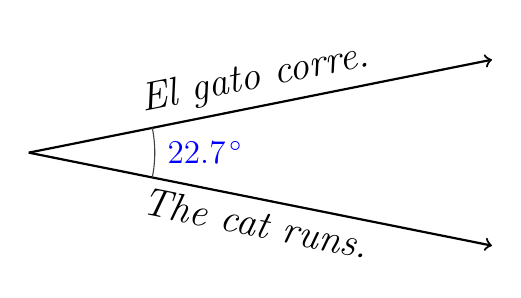
\begin{tikzpicture}[scale=6]
    \coordinate (O) at (0,0);
    \coordinate (A) at ({cos(\angledegrees/2)}, {-sin(\angledegrees/2)});
    \coordinate (B) at ({cos(\angledegrees/2)}, {sin(\angledegrees/2)});

    \draw[->, thick] (O) -- (A)
        node[midway, below left, sloped, anchor=north, font=\Large]
        {\textit{The cat runs.}};
    \draw[->, thick] (O) -- (B)
        node[midway, above left, sloped, anchor=south, font=\Large]
        {\textit{El gato corre.}};

    \pic [
        draw, darkgray, angle radius=1.6cm, angle eccentricity=1.4,
        "$\angledegrees^{\,\circ}$", text=blue, font=\large
    ] {angle=A--O--B};
\end{tikzpicture}

\end{document}
